%  !TeX  root  =  user_guide.tex

\chapter{Обзор возможностей}\label{feature_glance}

% when the revision of a section has been finalized,
% comment out the following line:
%\updatedisclaimer

После первого простого рабочего цикла в Разделе \ref{label_getstarted},
сделаем более детальный обзор возможностей QGIS. Большая часть
возможностей, представленных в последующих главах, будут объяснены и
описаны в руководстве позднее, в посвященных им разделах.

\section{Запуск и выход из QGIS}\label{label_startinqgis}

В разделе~\ref{samplesession} вы узнали как запустить QGIS. Повторим это
здесь и вы увидите, что QGIS предоставляет дополнительные параметры
командной строки.

\begin{itemize}
\item \nix{Предполагая, что QGIS установлен в PATH, вы можете запустить
QGIS набрав в командной строке: \usertext{qgis} или двойным нажатием на ссылке (или ярлыке) QGIS на
рабочем столе или в меню Приложения.}
\item \win{Запустите QGIS через меню Пуск или через ярлык на рабочем столе, или дважды нажав на
значке файла проекта QGIS.}
\item \osx{Дважды нажмите значок в вашей папке Приложения. Если необходимо запустить QGIS в
оболочке, выполните /path-to-installation-executable/Contents/MacOS/Qgis.}
\end{itemize}

Для выхода из QGIS, нажмите меню \{\nix{}\win{Файл} \osx{QGIS}\} > Выход,или используйте
комбинацию клавиш \keystroke{Ctrl+Q}.

\subsection{Параметры командной строки}\index{command line options}
\label{label_commandline}

\nix QGIS поддерживает множество параметров при запуске из командной строки. Для получения полного
списка параметров, введите в командной строке \usertext{qgis ---help}. В результате мы получим:

\small
\begin{verbatim}
qgis --help
Quantum GIS - 1.5.0-Tethys 'Tethys' (exported)
Quantum GIS (QGIS) is a viewer for spatial data sets, including
raster and vector data.
Usage: qgis [options] [FILES]
  options:
        [--snapshot filename]           emit snapshot of loaded datasets to given file
        [--width width]                 width of snapshot to emit
        [--height height]               height of snapshot to emit
        [--lang language]               use language for interface text
        [--project projectfile]         load the given QGIS project
        [--extent xmin,ymin,xmax,ymax]  set initial map extent
        [--nologo]                      hide splash screen
        [--help]                        this text

  FILES:
    Files specified on the command line can include rasters,
    vectors, and QGIS project files (.qgs):
     1. Rasters - Supported formats include GeoTiff, DEM
        and others supported by GDAL
     2. Vectors - Supported formats include ESRI Shapefiles
        and others supported by OGR and PostgreSQL layers using
        the PostGIS extension
\end{verbatim}
\normalsize

\begin{Tip} \caption{\textsc{Пример использования параметров командной строки}}
Можно запускать QGIS, указав в командной строке один или несколько файлов данных. Например, полагая,
что командная строка выполняется в директории qgis\_sample\_data, можно запустить QGIS с загрузкой
в него уже при старте векторного и растрового слоев, используя следующую команду:
\usertext{qgis ./raster/landcover.img ./gml/lakes.gml}
\end{Tip}

\minisec{Параметр командной строки \usertext{---snapshot}}
Этот параметр позволяет создавать снимок текущего вида в формате PNG. Это может быть удобно при
большом количестве проектов и необходимости создания снимков имеющихся данных.

При использовании в таком виде, создается PNG-файл с размерами 800x600 пикселей. Можно адаптировать, используя аргументы командной строки \usertext{---width} и \usertext{---height}. Имя файла задается после \usertext{---snapshot}.

\minisec{Параметр командной строки \usertext{---lang}}
Основываясь на языковых настройках операционной системы, QGIS выбирает соответствующий язык интерфейса пользователя (локализацию). Если хотите сменить локализацию интерфейса, можете задать языковой
код. Например: \usertext{---lang=it} запускает QGIS с итальянской локализацией. Список поддерживаемых в настоящее время языков с их кодами и статусом можно уточнить на веб-странице
\url{http://www.qgis.org/wiki/GUI_Translation_Progress}

\minisec{Параметр командной строки \usertext{---project}}
Также возможно запустить QGIS с существующим файлом проекта. Просто добавьте параметр
\usertext{---project} после имени проекта и QGIS запустится с открытыми слоями описанными в данном
файле проекта.

\minisec{Параметр командной строки \usertext{---extent}}
Используйте этот параметр для запуска с определенным охватом карты. Необходимо добавить прямоугольник
охвата, в следующем порядке, значения разделяются запятой:
\begin{verbatim}
--extent xmin,ymin,xmax,ymax
\end{verbatim}

\minisec{параметр командной строки \usertext{---nologo}}
Этот аргумент командной строки скрывает окно приветствия при запуске QGIS.

\section{Интерфейс QGIS}\index{main window}
\label{label_qgismainwindow}

Когда QGIS запущен, вы видите графический интерфейс пользователя (Graphical user interface, GUI),
как показано далее (номера с 1 по 6 в желтых овалах, ссылаются на шесть основных областей
интерфейса, как описано ниже):

\begin{figure}[ht]
   \centering
    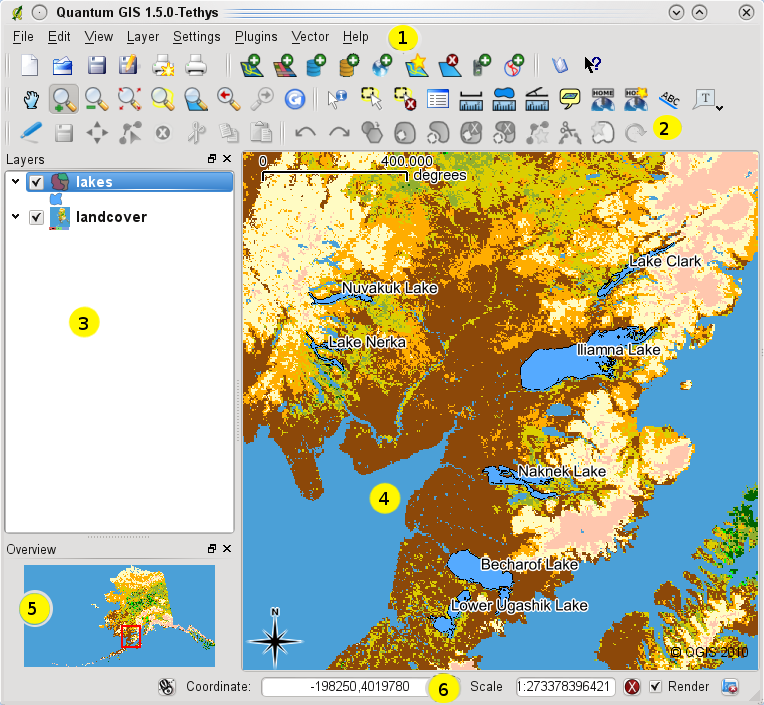
\includegraphics[clip=true, width=12cm]{startup}
    \caption{Интерфейс QGIS с открытым примером данных Alaska \nixcaption (KDE)} \label{fig:startup}
\end{figure}

\textbf{Примечание:} Внешний вид элементов интерфейса (заголовки и т.п.) может отличаться, в
зависисмости от операционной системы и менеджера окон.\\

Интерфейс QGIS разделяется на шесть областей:

\begin{tabular}{p{5cm} p{5cm}}
%\centering
1. Панель меню & 4. Окно карты \\
2. Панель инструментов & 5. Обзорная карта \\
3. Легенда карты & 6. Строка состояния \\
\end{tabular}

Более детально, эти шесть компонентов интерфейса QGIS, описаны в следующих разделах. Еще два раздела
описывают комбинации клавиш и контекстную справку.
% \newpage

\subsection{Панель меню}\label{label_menubar}
\index{menus}

Панель меню предоставляет доступ к разнообразным возможностям QGIS, используя стандартное иерархическое меню. Ниже показаны меню верхнего уровня и краткое описание их содержимого, вместе со значками
 соответствующих им инструментов, по мере их появления на панели интрементов, а также комбинации
 клавиш клавиатуры.\footnote{Комбинации клавиш могут быть настроены вручную (комбинации, показанные
 в этом разделе, используются по-умолчанию), используя инструмент Комбинации клавиш в меню Установки.}
Несмотря на то, что большинству пунктов меню соответствует свой инструмент (и наоборот), меню и
панели инструментов организованы не совсем одинаково. Панель инструментов, в которой находится
инструмент, показана после каждого пункта меню как флажок. Дополнительную информацию об инструментах
и панелях инструментов можно найти в Разделе \ref{label_toolbars}.

\begin{tabbing}
\hspace{5.5cm}\=\hspace{3cm}\=\hspace{3.5cm}\= \kill
\hspace{1cm} Пункт меню \> Комбинация клавиш \> Справка \> Панель инструментов\\
\end{tabbing}

\begin{itemize}
\item \mainmenuopt{Файл}
\begin{tabbing}
\hspace{4.5cm}\=\hspace{3cm}\=\hspace{3.5cm}\= \kill
\dropmenuopttwo{mActionFileNew}{Новый проект}
	\> \keystroke{Ctrl+N}
	\> см. Раздел \ref{sec:projects}
	\> \dropmenucheck{Файл} \\
\dropmenuopttwo{mActionFileOpen}{Открыть проект}
	\> \keystroke{Ctrl+O}
	\> см. Раздел \ref{sec:projects}
	\> \dropmenucheck{Файл} \\
\dropmenuopt{Открыть недавние проекты}
	\>
	\> см. Раздел \ref{sec:projects} \\
\dropmenuopttwo{mActionFileSave}{Сохранить проект}
	\> \keystroke{Ctrl+S}
	\> см. Раздел \ref{sec:projects}
	\> \dropmenucheck{Файл} \\
\dropmenuopttwo{mActionFileSaveAs}{Сохранить проект как...}
	\> \keystroke{Ctrl+Shift+S}
  \> см. Раздел \ref{sec:projects}
	\> \dropmenucheck{Файл} \\
\dropmenuopttwo{mActionSaveMapAsImage}{Сохранить как изображение}
	\>
	\> см. Раздел \ref{sec:output} \\
\dropmenuopttwo{mActionNewComposer}{Создать компоновку карты}
        \> \keystroke{Ctrl+P}
        \> см. Раздел \ref{label_printcomposer}
        \> \dropmenucheck{Файл} \\
\dropmenuopttwo{mActionComposerManager}{Управление компоновками}
	\>
	\> см. Раздел \ref{label_printcomposer}
	\> \dropmenucheck{Файл} \\
\dropmenuopt{Компоновки карт}
	\>
	\> см. Раздел \ref{label_printcomposer} \\
\dropmenuopttwo{mActionFileExit}{Выход}
	\> \keystroke{Ctrl+Q} \\
\end{tabbing}

\item \mainmenuopt{Правка}
\begin{tabbing}
\hspace{4.5cm}\=\hspace{3cm}\=\hspace{3.5cm}\= \kill
\dropmenuopttwo{mActionUndo}{Отменить}
        \> \keystroke{Ctrl+Z}
        \> см. Раздел \ref{sec:advanced_edit}
        \> \dropmenucheck{Дополнительные функции оцифровки} \\
\dropmenuopttwo{mActionRedo}{Вернуть}
        \> \keystroke{Ctrl+Shift+Z}
        \> см. Раздел \ref{sec:advanced_edit}
        \> \dropmenucheck{Дополнительные функции оцифровки} \\
\dropmenuopttwo{mActionEditCut}{Вырезать объекты}
	\> \keystroke{Ctrl+X}
	\> см. Раздел \ref{sec:edit_existing_layer}
	\> \dropmenucheck{Оцифровка} \\
\dropmenuopttwo{mActionEditCopy}{Копировать объекты}
	\> \keystroke{Ctrl+C}
	\> см. Раздел \ref{sec:edit_existing_layer}
	\> \dropmenucheck{Оцифровка} \\
\dropmenuopttwo{mActionEditPaste}{Вставить объекты}
	\> \keystroke{Ctrl+V}
	\> см. Раздел \ref{sec:edit_existing_layer}
	\> \dropmenucheck{Оцифровка} \\
\dropmenuopttwo{mActionEditPaste}{Переместить объект}
        \>
        \> см. Раздел \ref{sec:edit_existing_layer}
        \> \dropmenucheck{Оцифровка} \\
\dropmenuopttwo{mActionDeleteSelected}{Удалить выделенное}
        \>
        \> см. Раздел \ref{sec:edit_existing_layer}
        \> \dropmenucheck{Оцифровка} \\
\dropmenuopttwo{mActionSimplify}{Упростить объект}
        \>
        \> см. Раздел \ref{sec:advanced_edit}
        \> \dropmenucheck{Дополнительные функции оцифровки} \\
\dropmenuopttwo{mActionAddRing}{Добавить кольцо}
        \>
        \> см. Раздел \ref{sec:advanced_edit}
        \> \dropmenucheck{Дополнительные функции оцифровки} \\
\dropmenuopttwo{mActionAddIsland}{Добавить часть}
        \>
        \> см. Раздел \ref{sec:advanced_edit}
        \> \dropmenucheck{Дополнительные функции оцифровки} \\
\dropmenuopttwo{mActionDeleteRing}{Удалить кольцо}
        \>
        \> см. Раздел \ref{sec:advanced_edit}
        \> \dropmenucheck{Дополнительные функции оцифровки} \\
\dropmenuopttwo{mActionDeletePart}{Удалить часть}
        \>
        \> см. Раздел \ref{sec:advanced_edit}
        \> \dropmenucheck{Дополнительные функции оцифровки} \\
\dropmenuopttwo{mActionReshape}{Корректировать объекты}
        \>
        \> см. Раздел \ref{sec:advanced_edit}
        \> \dropmenucheck{Дополнительные функции оцифровки} \\
\dropmenuopttwo{mActionSplitFeatures}{Разбить объекты}
        \>
        \> см. Раздел \ref{sec:advanced_edit}
        \> \dropmenucheck{Дополнительные функции оцифровки} \\
\dropmenuopttwo{mActionMergeFeatures}{Объединить выбранные объекты}
        \>
        \> см. Раздел \ref{sec:advanced_edit}
        \> \dropmenucheck{Дополнительные функции оцифровки} \\
\dropmenuopttwo{mActionNodeTool}{Редактирование узлов}
        \>
        \> см. Раздел \ref{sec:edit_existing_layer}
        \> \dropmenucheck{Оцифровка} \\
\dropmenuopttwo{mActionRotatePointSymbols}{Повернуть значки}
        \>
        \> см. Раздел \ref{sec:advanced_edit}
        \> \dropmenucheck{Дополнительные функции оцифровки} \\
\end{tabbing}

После активации \toolbtntwo{mActionToggleEditing}{Режим редактирования} для слоя, в меню
\mainmenuopt{Правка} появится значок создания объекта, в зависимости от типа слоя (точечный,
линейный или полигональный). \\

\begin{tabbing}
\hspace{4.5cm}\=\hspace{3cm}\=\hspace{3.5cm}\= \kill
\dropmenuopttwo{mActionCapturePoint}{Создать точку}
        \>
        \> см. Раздел \ref{sec:edit_existing_layer}
        \> \dropmenucheck{Оцифровка} \\
\dropmenuopttwo{mActionCaptureLine}{Создать линию}
        \>
        \> см. Раздел \ref{sec:edit_existing_layer}
        \> \dropmenucheck{Оцифровка} \\
\dropmenuopttwo{mActionCapturePolygon}{Создать полигон}
        \>
        \> см. Раздел \ref{sec:edit_existing_layer}
        \> \dropmenucheck{Оцифровка} \\
\end{tabbing}


\item \mainmenuopt{Вид}
\begin{tabbing}
\hspace{4.5cm}\=\hspace{3cm}\=\hspace{3.5cm}\= \kill
\dropmenuopttwo{mActionPan}{Прокрутка карты}
	\>
	\> \> \dropmenucheck{Навигация} \\
\dropmenuopttwo{mActionZoomIn}{Увеличить}
	\> \keystroke{Ctrl++}
	\> \> \dropmenucheck{Навигация} \\
\dropmenuopttwo{mActionZoomOut}{Уменьшить}
	\> \keystroke{Ctrl+-}
	\> \> \dropmenucheck{Навигация} \\
\dropmenuopttwo{mActionSelect}{Выбрать объекты}
	\>
	\> \> \dropmenucheck{Атрибуты} \\
\dropmenuopttwo{mActionDeselectAll}{Снять выделение во всех слоях}
        \>
        \> \> \dropmenucheck{Атрибуты} \\
\dropmenuopttwo{mActionIdentify}{Определить объекты}
	\> \keystroke{Ctrl-Alt-I}
	\> \> \dropmenucheck{Атрибуты} \\
\dropmenuopttwo{mActionMeasure}{Измерить линию}
	\> \keystroke{Ctrl-Alt-M}
	\> \> \dropmenucheck{Атрибуты} \\
\dropmenuopttwo{mActionMeasureArea}{Измерить площадь}
	\> \keystroke{Ctrl-Alt-J}
	\> \> \dropmenucheck{Атрибуты} \\
\dropmenuopttwo{mActionMeasureAngle}{Измерить угол}
	\>
	\> \> \dropmenucheck{Атрибуты} \\
\dropmenuopttwo{mActionOpenTable}{Полный охват}
	\> \keystroke{Ctrl-Alt-F}
	\> \> \dropmenucheck{Навигация} \\
\dropmenuopttwo{mActionZoomToLayer}{Увеличить до слоя}
	\>
	\> \> \dropmenucheck{Навигация} \\
\dropmenuopttwo{mActionZoomToSelected}{Увеличить до выделенного}
	\> \keystroke{Ctrl+J}
	\> \> \dropmenucheck{Навигация} \\
\dropmenuopttwo{mActionZoomLast}{Предыдущий охват}
	\>
	\> \> \dropmenucheck{Навигация} \\
\dropmenuopttwo{mActionZoomNext}{Следующий охват}
	\>
	\> \> \dropmenucheck{Навигация} \\
\mainmenuopt{Фактический размер}
	\>
	\> \>  \\
\dropmenuopttwo{mActionMapTips}{Всплывающие описания}
	\>
	\> \> \dropmenucheck{Атрибуты} \\
\dropmenuopttwo{mActionNewBookmark}{Новая закладка}
	\> \keystroke{Ctrl+B}
	\> см. Раздел \ref{sec:bookmarks}
\> \dropmenucheck{Атрибуты} \\
\dropmenuopttwo{mActionShowBookmarks}{Показать закладки}
	\> \keystroke{Ctrl-Alt-B}
	\> см. Раздел \ref{sec:bookmarks}
	\> \dropmenucheck{Атрибуты} \\
\dropmenuopttwo{mActionDraw}{Обновить}
	\> \keystroke{Ctrl+R}
	\> \> \dropmenucheck{Навигация} \\
\mainmenuopt{Уровень детализации}
	\>
	\> см. Раздел \ref{sec:tilesets}
	\> \dropmenucheck{Уровень детализации} \\
\mainmenuopt{GPS-слежение}
	\>
	\> см. Раздел \ref{sec:gpstracking}
	\> \dropmenucheck{GPS слежение} \\
\end{tabbing}

\item \mainmenuopt{Слой}
\begin{tabbing}
\hspace{5cm}\=\hspace{3cm}\=\hspace{3.5cm}\= \kill
\dropmenuopt{Создать}
	\>
	\> см. Раздел \ref{sec:create shape}
	\> \dropmenucheck{Управление слоями} \\
\dropmenuopttwo{mActionAddNonDbLayer}{Добавить векторный слой}
	\> \keystroke{Ctrl+Shift+V}
	\>
	см. Раздел \ref{label_workingvector}
	\> \dropmenucheck{Управление слоями} \\
\dropmenuopttwo{mActionAddRasterLayer}{Добавить растровый слой}
	\> \keystroke{Ctrl+Shift+R}
	\>
	см. Раздел \ref{label_raster}
	\> \dropmenucheck{Управление слоями} \\
\dropmenuopttwo{mActionAddLayer}{Добавить слой PostGIS}
	\> \keystroke{Ctrl+Shift+D}
	\>
	см. Раздел \ref{label_postgis}
        \> \dropmenucheck{Управление слоями} \\
\dropmenuopttwo{mActionAddSpatiaLiteLayer}{Добавить слой SpatiaLite}
        \> \keystroke{Ctrl+Shift+L}
        \>
        см. Раздел \ref{label_spatialite}
	\> \dropmenucheck{Управление слоями} \\
\dropmenuopttwo{mActionAddWmsLayer}{Добавить WMS-слой}
	\> \keystroke{Ctrl+Shift+W}
	\>
	см. Раздел \ref{sec:ogc-wms}
	\> \dropmenucheck{Управление слоями} \\
\dropmenuopttwo{mActionOpenTable}{Открыть таблицу атрибутов}
	\> \>
	\> \dropmenucheck{Атрибуты} \\
\dropmenuopttwo{mActionFileSave}{Сохранить изменения}
        \> \>
        \> \dropmenucheck{Оцифровка} \\
\dropmenuopttwo{mActionToggleEditing}{Режим редактирования}
	\> \>
	\> \dropmenucheck{Оцифровка} \\
\mainmenuopt{Сохранить как...}
	\\
\mainmenuopt{Сохранить выделение как...}
	\\
\dropmenuopttwo{mActionRemoveLayer}{Удалить слой}
	\> \keystroke{Ctrl+D}
	\>
	\> \dropmenucheck{Управление слоями} \\
\mainmenuopt{Свойства}
	\\
\mainmenuopt{Запрос...}
	\\
\dropmenuopttwo{mActionInOverview}{Добавить в обзор}
	\> \keystroke{Ctrl+Shift+O}
	\\
\dropmenuopttwo{mActionAddAllToOverview}{Добавить все в обзор}
	\\
\dropmenuopttwo{mActionRemoveAllFromOverview}{Удалить все из обзора}
	\\
\dropmenuopttwo{mActionHideAllLayers}{Скрыть все слои}
	\> \keystroke{Ctrl+Shift+H}
	\\
\dropmenuopttwo{mActionShowAllLayers}{Показать все слои}
	\> \keystroke{Ctrl+Shift+U}
	\\
\dropmenuopttwo{labeling}{Подписи}
	\> \>
	\> \dropmenucheck{Атрибуты} \\
\end{tabbing}

\item \mainmenuopt{Установки}
\begin{tabbing}
\hspace{5cm}\=\hspace{3cm}\=\hspace{3.5cm}\= \kill
\dropmenuopt{Панели}
	\>
	\>
	\\
\dropmenuopt{Панели инструментов}
	\>
	\>
	\\
\mainmenuopt{Полноэкранный режим}
	\>\keystroke{Ctrl-F}
	\>
	\\
\dropmenuopttwo{mActionProjectProperties}{Свойства проекта}
	\> \keystroke{Ctrl-Alt-P}
	\> см. Раздел \ref{sec:projects} \\
\dropmenuopttwo{mActionCustomProjection}{Ввод системы координат}
        \> \> см. Раздел \ref{sec:customprojections} \\
\mainmenuopt{Управление стилями}
        \> \> \\
\dropmenuopttwo{mActionOptions}{Комбинации клавиш}
        \> \> \\
\dropmenuopttwo{mActionOptions}{Параметры}
        \> \> см. Раздел \ref{subsec:gui_options} \\
\end{tabbing}

\item \mainmenuopt{Модули} - (Следующие пункты меню добавляются подключаемыми модулями после их загрузки.)
\begin{tabbing}
\hspace{5cm}\=\hspace{3cm}\=\hspace{3.5cm}\= \kill
\dropmenuopttwo{mActionShowPluginManager}{Управление модулями}
	\> \> см. Раздел \ref{sec:managing_plugins} \dropmenucheck{Модули}
	\\
	\mainmenuopt{Консоль Python}
        \> \>
        \\
\end{tabbing}

\item \mainmenuopt{Справка}
\begin{tabbing}
\hspace{5cm}\=\hspace{3cm}\=\hspace{3.5cm}\= \kill
\dropmenuopttwo{mActionHelpContents}{Содержание}
	\> \keystroke{F1}
	\>
	\> \dropmenucheck{Справка}\\
\dropmenuopttwo{mActionQgisHomePage}{Веб-сайт QGIS}
	\> \keystroke{Ctrl+H}
	\>
	\\
\dropmenuopttwo{mActionCheckQgisVersion}{Проверить версию QGIS}
	\\
\dropmenuopttwo{mActionHelpAbout}{О программе}
	\\
\end{tabbing}

\end{itemize}

\textbf{Примечание:} \nix Пункты панели меню, перечисленные выше, являются стандартными для менеджера окон в KDE. В GNOME, меню Установки отсутствует, а его пункты расположены следующим образом:
\begin{tabbing}
\dropmenuopttwo{mActionProjectProperties}{Свойства проекта} \hspace{3cm}\=
\dropmenucheck{Файл} \\
\dropmenuopttwo{mActionOptions}{Параметры} \hspace{3cm}\>
\dropmenucheck{Правка}\\
\dropmenuopttwo{mActionOptions}{Комбинации клавиш} \hspace{3cm}\>
\dropmenucheck{Правка}\\
\mainmenuopt{Управление стилями} \hspace{3cm}\>
\dropmenucheck{Правка}\\
\dropmenuopttwo{mActionCustomProjection}{Ввод системы координат}\hspace{3cm}\>
\dropmenucheck{Правка} \\
\dropmenuopt{Панели} \hspace{3cm}\>
\dropmenucheck{Вид} \\
\dropmenuopt{Панели инструментов}   \hspace{3cm}\>
\dropmenucheck{Вид} \\
\mainmenuopt{Полноэкранный режим} \hspace{3cm}\>
\dropmenucheck{Вид} \\
\mainmenuopt{Уровень детализации} \hspace{3cm}\>
\dropmenucheck{Вид} \\
\mainmenuopt{GPS-слежение} \hspace{3cm}\>
\dropmenucheck{Вид} \\
\end{tabbing}

%See Appendix \ref{app_menu} for complete descriptions of the menu items.

\subsection{Панели инструментов}\label{label_toolbars}
\index{toolbars}

Панели инструментов обеспечивают доступ к большинству из тех же функций, что и меню, а также
содержат дополнительные инструменты для работы с картой. Для каждого пункта панели инструментов, также доступна всплывающая подсказка. Задержите мышь над пунктом панели инструментов и отобразится
краткое описание назначения инструмента.

Каждую панель инструментов можно перемещать в зависимости от ваших потребностей. Кроме того,
каждую панель инструментов можно скрыть при помощи контекстного меню, появляюшегося при нажатии
правой кнопкой мыши на панели инструментов.

\begin{Tip}
\caption{\textsc{Восстановление панелей инструментов}} \index{layout!toolbars}
Если вы случайно скрыли все панели инструментов, можно вернуть их обратно, используя пункт меню
 \mainmenuopt{Вид} > \dropmenuopt{Панели инструментов}.
\end{Tip}

\subsection{Легенда карты}\label{label_legend}
\index{legend}

Область легенды карты предназначена для установки видимости и порядка расположения слоев карты.
Порядок расположения слоев означает, что слои находящиеся ближе к верхней части легенды,
отрисовываются в окне карты над слоями, перечисленными в легенде ниже. Флажок у каждого пункта
легенды, используется для показа или скрытия слоя.\index{layer!visibility}

Слои могут быть сгруппированы в окне легенды путем добавления группы слоев и перетаскивания слоев в
группу. Для этого, поместите курсор мыши в окне легенды карты, нажмите правую кнопку мыши, выберите
 \dropmenuopt{Добавить группу}. Появится новая папка. Теперь, перетащите слои на значок папки. Это
дает возможность переключать видимость всех слоев в группе одним нажатием. Для вывода слоев из
группы, нажмите правой кнопкой мыши на значке слоя и выберите \dropmenuopt{Сделать элементом первого уровня}. Чтобы переименовать папку, выберите \dropmenuopt{Переименовать}, нажав правой кнопкой
на имени группы.

Содержание контекстного меню, доступного при нажатии правой кнопки мыши на слое,зависит от того,
на каком слое в окне легенды вы нажали правой кнопкой"---растровом или векторном. Для векторных
слоев GRASS \dropmenuopt{Режим редактирования} недоступен. Для дополнительной информации по
редактированию векторных слоев GRASS, см. Раздел \ref{grass_digitising}.

\begin{itemize}

\item \textbf{Меню правой кнопки мыши для растровых слоев}
\begin{itemize}
\item \dropmenuopt{Увеличить до границ слоя}
\item \dropmenuopt{Увеличить до наилучшего масштаба (100\%)}
\item \dropmenuopt{Показать в обзоре}
\item \dropmenuopt{Удалить}
\item \dropmenuopt{Свойства}
\item \dropmenuopt{Переименовать}
\item \dropmenuopt{Добавить группу}
\item \dropmenuopt{Развернуть все}
\item \dropmenuopt{Свернуть все}
%%\item \dropmenuopt{Show file groups}
\end{itemize}

\item \textbf{Меню правой кнопки мыши для векторных слоев}
\begin{itemize}
\item \dropmenuopt{Увеличить до границ слоя}
\item \dropmenuopt{Показать в обзоре}
\item \dropmenuopt{Удалить}
\item \dropmenuopt{Открыть таблицу атрибутов}
\item \dropmenuopt{Режим редактирования (недоступен для слоев GRASS)}
\item \dropmenuopt{Сохранить как...}
\item \dropmenuopt{Сохранить выделение как...}
\item \dropmenuopt{Запрос}
\item \dropmenuopt{Свойства}
%% \item \dropmenuopt{Make to toplevel item}
\item \dropmenuopt{Переименовать}
\item \dropmenuopt{Добавить группу}
\item \dropmenuopt{Развернуть все}
\item \dropmenuopt{Свернуть все}
%%\item \dropmenuopt{Show file groups}
\end{itemize}

\item \textbf{Меню правой кнопки мыши для групп слоев}
\begin{itemize}
\item \dropmenuopt{Удалить}
\item \dropmenuopt{Переименовать}
\item \dropmenuopt{Добавить группу}
\item \dropmenuopt{Развернуть все}
\item \dropmenuopt{Свернуть все}
%%\item \dropmenuopt{Show file groups}
\end{itemize}

\end{itemize}

В случае, если несколько источников векторных данных имеют одинаковый тип вектора и те же атрибуты,
их символика может быть сгруппирована. Это означает, что если символика одного источника данных
изменится, другие автоматически получат новую символику. Для группировки символики, откройте меню правой кнопки мыши в окне легенды и выберите \dropmenuopt{Добавить группу}. Появится файл группы слоев.
Стало возможным перетаскивание файла из одной группы в другую. Если это будет сделано, символика будет сгруппирована. Обратите внимание, что QGIS позволяет перетаскивание, только если два слоя имеют
возможность обмениваться символикой (тот же тип векторной геометрии и те же атрибуты).

%% isn't included in Titan anymore, except for an "toggle overview"
%Each legend entry can show the following mini icons:
%
%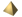
\includegraphics[width=0.7cm]{pyramid} This is a raster
%that has pyramids built for it to improve rendering efficiency (see
%Section \ref{raster_pyramids}).\\
%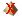
\includegraphics[width=0.7cm]{no_pyramid} This is a
%raster that has no pyramid layers (see Section \ref{raster_pyramids}).\\
%
\includegraphics[width=0.7cm]{inoverview} This layer is
%shown in the overview map area as well as in the main map window.\\
%
\includegraphics[width=0.7cm]{editable} This is a vector
%layer that is currently enabled for editing.\\

\subsection{Окно карты}\label{label_mapview}
\index{map!view}

Это наиболее важная часть QGIS"---в этом окне отображаются карты! Карта, отображаемая в этом окне,
зависит от того, какие векторные и растровые слои загружены в QGIS (см. разделы для получения
дополнительной информации о загрузке слоев). Данные в окне карты можно панорамировать (прокручивать,
смещать фокус отображения карты на другую область) и масштабировать (увеличивать или уменьшать). Также с картой можно выполнять многие другие операции, как было описано выше про панели инструментов. Окно карты и легенда тесно связаны друг с другом"---карта отображает изменения, вносимые в области легенды.

\begin{Tip}\caption{\textsc{Масштабирование карты с помощью колеса мыши}}\index{zoom!mouse wheel}
Можно использовать колесо мыши для увеличения и уменьшения масштаба карты. Поместите курсор мыши
внутри окна карты и вращайте колесо вперед (от себя) для увеличения масштаба (приближения)и назад
для уменьшения масштаба (удаления). Масштабирование производится относительно центра, которым
является положение курсора мыши. Поведение колеса мыши при масштабировании, можно настроить по
своему вкусу, используя вкладку \tab{Инструменты} в меню \mainmenuopt{Установки} >
\dropmenuopt{Праметры}.
\end{Tip}

\begin{Tip}\caption{\textsc{Панорамирование карты, используя клавиши со стрелками и клавишу
пробела}}\index{pan!arrow keys}
Можно использовать клавиши со стрелками для панорамирования (прокрутки) карты. Поместите курсор мыши внутри окна карты, нажмите на клавишу вправо клавиатуры для панорамирования на восток, влево"---для панорамирования на запад, вверх"---для панорамирования на север и вниз"---для панорамирования на юг.
Также можно панорамировать карту используя клавишу пробел: просто передвигайте курсор с нажатой клавишей пробела.
\end{Tip}

\subsection{Обзорная карты}\label{label_mapoverview}
\index{map!overview}

Панель Обзора (или обзорная карта) предоставляет вид полного охвата слоев добавленых в обзор. Панель обзора можно включить через меню \mainmenuopt{Вид} >\dropmenuopt{Панели}. Внутри окна обзора находится прямоугольник, отображающий текущий охват карты. Это позволяет быстро определять, какая область карты сейчас просматривается в окне карты. Обратите внимание, что подписи в окне обзора не отображаются, даже если слои настроены для подписывания.

Добавить в Обзор единичный слой можно, нажав правой кнопкой мыши на этом слое в легенде и выбрав \checkbox{Показать в обзоре}. Также можно добавлять и удалять слои из обзорной карты, используя соответствующие пункты в меню Слой.

Если нажать и переместить красный прямоугольник в обзорной карте,показывающий текущий охват, окно карты соответственно обновится.

\subsection{Строка состояния}\label{label_statusbar}

Строка состояния отображает текущую позицию в координатах карты (например, в метрах или десятичных градусах) курсора мыши при его перемещении в окне карты. Слева от отображаемых координат в строке состояния, находится маленькая кнопка, которая позволяет переключаться между отображением координат позиции курсора и координат границ вывода карты при масштабировании и панорамировании.

Индикатор выполнения в строке состояния, отображает процесс отрисовки (рендеринга) каждого слоя в окне карты. В некоторых случаях, таких как подсчет статистики в растровых слоях, индикатор состояния используется для отображения статуса длительных операций.

В случае, если будет доступен новый модуль или обновление для существующего модуля, в строке состояния появится новое сообщение. Справа в строке состояния, находится маленький флажок, который используется для временного прекращения отрисовки слоев в окне карты (см. Раздел \ref{subsec:redraw_events} ниже). Последним справа, в строке состояния, находится значок Преобразования координат. Нажатие на нем открывает диалоговое окно Системы координат текущего проекта.

\begin{Tip}\caption{\textsc{Вычисление правильного масштаба карты}}\index{scale!calculate}
При запуске QGIS, единицами измерения по-умолчанию являются градусы, и QGIS считает, что любые
координаты в вашем слое, также градусы. Для получения правильных значений масштаба, можно, либо вручную изменить единицы слоя на метры на вкладке \tab{Общие} пункта меню \mainmenuopt{Установки} >\dropmenuopt{Свойства проекта}, либо можно выбрать систему координат (CRS) нажатием на значке
\toolbtntwo{mIconProjectionDisabled}{Преобразование координат} в правом нижнем углу строки
состояния. В последнем случае, единицы слоя устанавливаются в соответствие с системой координат, например, '+units=m'.
\end{Tip}

\subsection{Комбинации клавиш}\label{shortcuts}
\index{Keyboard shortcuts}

QGIS предоставляет комбинации клавиш по-умолчанию для многих действий и инструментов. Их можно найти ниже, в Разделе \ref{label_menubar}. Дополнительно, пункт меню \mainmenuopt{Установки} >
\dropmenuopt{Комбинации клавиш} позволяет изменять комбинации клавиш назначенные по-умолчанию и добавлять новые комбинации для действий в QGIS.

\begin{figure}[ht]
   \centering
   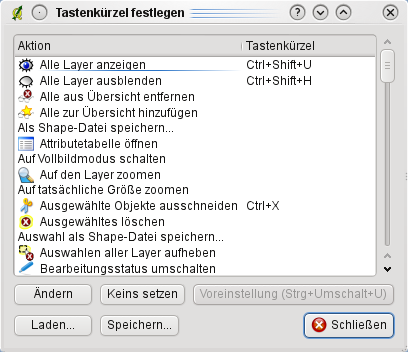
\includegraphics[clip=true, width=8cm]{shortcuts}
   \caption{Редактирование комбинаций клавиш \nixcaption (KDE)} \label{fig:shortcuts}
\end{figure}

Процесс редактирования комбинаций клавиш очень прост. Просто выберите действие или инструмент из списка и нажмите на кнопке \button{Изменить}, \button{Удалить} или \button{По умолчанию}. Единожды определив свою конфигурацию комбинаций клавиш, можно сохранить ее в файл XML и загрузить на другом компьютере с установленным QGIS.

\subsection{Контекстная справка}\label{context_help}
\index{Context help}

Если вам необходима помощь по конкретной теме, можно воспользоваться контекстной справкой по нажатию кнопки Справка, доступной в большинстве диалоговых окон, но, обратите внимание на то, что сторонние модули могут перенаправлять на справочные материалы размещенные в сети Интернет.

\section{Рендеринг}\label{subsec:redraw_events}\index{rendering}

По умолчанию, QGIS перерисовывает все видимые слои всякий раз, когда область отображения карты должна быть обновлена. События, запускающие процесс обновления карты,включают следующие:

\begin{itemize}
\item Добавление слоя
\item Панорамирование или масштабирование
\item Изменение размеров окна QGIS
\item Включение или отключение слоя (или слоев) в легенде
\end{itemize}

В ряде случаев, QGIS позволяет контролировать процесс рендеринга.

\subsection{Видимость в пределах масштаба}\index{rendering!scale dependent}
\label{label_scaledepend}

Видимость слоя в пределах масштаба, позволяет определить минимальный и максимальный масштабы, при которых слой будет видимым. Для включения видимости в пределах масштаба, откройте диалоговое окно \dialog{Свойства}, дважды нажав на слое в легенде. На вкладке \tab{Общие}, нажмите флажок \checkbox{Видимость в пределах масштаба} и установите значения минимального и максимального масштаба.

Можно задать значения масштабов, по первому масштабированию слоя, который вы хотите использовать, отмечая значение масштаба в строке состояния QGIS.\index{scale}

\subsection{Управление отрисовкой карты}\label{label_controlmap}

Отрисовка карты может контролироваться одним из следующих способов:

\minisec{a) Приостановка отрисовки}\index{rendering!suspending}
\label{label_suspendrender}

Для приостановки отрисовки карты, включите флажок \checkbox{Отрисовка} в правом нижнем углу строки состояния. Когда флажок \checkbox{Отрисовка} не включен, QGIS не будет перерисовывать карту в ответ на любое событие описанное в Разделе \ref{subsec:redraw_events}. Например, можно использовать приостановку отрисовки в следующих случаях:

\begin{itemize}
\item Добавление нескольких слоев сразу и задание символики перед нанесением на карту
\item Добавление одного или нескольких больших слоев и включение видимости в пределах масштаба перед нанесением на карту
\item Добавление одного или нескольких больших слоев и масштабирование к определенному виду перед нанесением на карту
\item Любая комбинация из вышеперечисленного
\end{itemize}

Включение флажка \checkbox{Отрисовка} активирует рендеринг и немедленно обновляет содержимое карты.

\minisec{b) Настройка параметра добавления слоя}\label{label_settinglayer}
\index{rendering!options}\index{layers!initial visibility}

Можно настроить параметр, позволяющий всегда загружать новые слои без отрисовки на карте. Это означает, что слой будет добавлен к карте, но флажок видимости, в легенде, не будет включен по умолчанию. Для настройки этого параметра, выберите пункт меню \mainmenuopt{Установки} > \dropmenuopt{Параметры} и нажмите на вкладке \tab{Отрисовка}. Выключите флажок \\\checkbox{Добавляемые на карту слои видимы по умолчанию}. Теперь, любой слой добавленный к карте, будет по умолчанию невидимым (выключенным).

%\minisec{Stopping Rendering}\index{rendering!halting}
%\label{label_stoprender}
%
%To stop the map drawing, press the ESC key. This will halt the refresh of
%the map canvas and leave the map partially drawn. It may take a bit of time
%between pressing ESC and the time the map drawing is halted.
%
%\textbf{NOTE}: It is currently not possible to stop rendering - this was disabled
%in qt4 port because of User Interface (UI) problems and crashes.

\minisec{c) Обновление окна карты во время отрисовки}
\label{label_updatemap}\index{rendering!update during drawing}

Можно настроить параметр обновления карты во время прорисовки объектов. По умолчанию, QGIS не отображает никаких объектов слоя на карте до тех пор, пока не отрисуется весь слой. Для обновления окна карты во время чтения из хранилища данных,выберите пункт меню \mainmenuopt{Установки} > \dropmenuopt{Параметры}, нажмите на вкладке \tab{Отрисовка}. Установите число объектов в соответствующее значение для обновления карты во время отрисовки. Установка значения равным 0, запрещает обновление карты во время отрисовки слоя (установлено по умолчанию). Установка слишком низкого значения,
скажется на производительности"---окно карты будет постоянно обновляться во время чтения объектов из хранилища. Приемлемое значение начинается с 500.

\minisec{d) Регулирование качества отрисовки}
\label{label_renderquality}\index{rendering!quality}

Для регулирования качества отрисовки карты, можно задать 2 параметра. Выберите пункт меню \mainmenuopt{Установки} > \dropmenuopt{Параметры}, нажмите на вкладке \tab{Отрисовка} и включите или отключите следующие флажки.

\begin{itemize}
\item \checkbox{Рисовать сглаженные линии (снижает скорость отрисовки)}
\item \checkbox{Исправлять ошибки заливки полигонов}
\end{itemize}

\section{Измерения}\label{sec:measure}\index{measure}

Измерения на карте работают только с Прямоугольными системами координат (например, UTM). Если загруженная карта определена с помощью Географической системы координат (широта/долгота), результаты измерений длин или площадей будут неправильными. Для исправления этого, необходимо настроить соответствующую систему координат карты (см. Раздел~\ref{label_projections}). Оба измерительных модуля также используют параметры прилипания из модуля оцифровки. Это может пригодиться, если необходимо провести измерения вдоль линии или площадного объекта в векторных слоях.

\subsection{Измерение длин, площадей и углов}
\index{measure:line length}
\index{measure:areas}
\index{measure:angles}

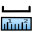
\includegraphics[width=0.7cm]{mActionMeasure}
QGIS позволяет измерить реальное расстояние между заданными точками в соответствии с определенным эллипсоидом. Для настройки, выберите пункт меню \mainmenuopt{Установки} > \dropmenuopt{Параметры},
нажмите на вкладке \tab{Инструменты} и выберите соответствующий эллипсоид. Там же можно выбрать цвет линии и единицы измерения по умолчанию (метры или футы). Используя инструмент, нажимайте на карте, ставя на ней точки. Длина каждого сегмента, а также общий результат, отображается в окне измерений. Чтобы остановить измерения, нажмите правую кнопку мыши. \\

\includegraphics[width=0.7cm]{mActionMeasureArea} Также можно измерять площади. В окне измерений появится итоговый размер области  \\
Кроме того, инструмент измерений будет прилипать к объектам выбранного слоя, при условии, что для слоя установлен порог прилипания. (см. Раздел~\ref{snapping_tolerance}). Итак, если необходимо измерить точно вдоль линейного объекта, или вокруг полигонального объекта, необходимо настроить порог прилипания, а затем выбрать слой. Теперь, при использовании инструмента измерений, при каждом нажатии кнопки мыши (в пределах порога прилипания), курсор будет прилипать к объектам этого слоя. \\
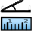
\includegraphics[width=0.7cm]{mActionMeasureAngle}
Также, вы можете измерять углы, выбрав инструмент Измерить угол. Курсор станет крестообразным. Нажмите для создания первого сегмента угла, который хотите измерить, затем перемещайте курсор для создания желаемого угла. Результат измерения отображается во всплывающем диалоговом окне.

\begin{figure}[ht]
\centering
   \subfloat[Измерение линий] {\label{subfig:measure_line}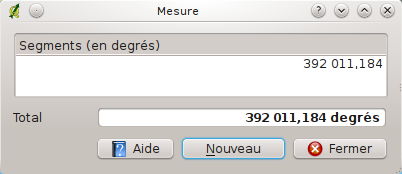
\includegraphics[clip=true, width=0.3\textwidth]{measure_line}}
     \hspace{0.33cm}
   \subfloat[Измерение площадей]{\label{subfig:measure_area}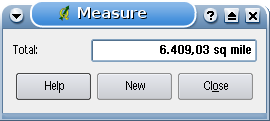
\includegraphics[clip=true, width=0.3\textwidth]{measure_area}}
     \hspace{0.33cm}
   \subfloat[Измерение углов]{\label{subfig:measure_angle}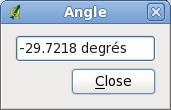
\includegraphics[clip=true, width=0.3\textwidth]{measure_angle}}
   \caption{Инструменты измерений \nixcaption} \label{fig:measure}
\end{figure}


\section{Проекты}\label{sec:projects}\index{projects}

Состояние вашего сеанса, QGIS рассматривается как Проект. Одновременно, QGIS работает с одним проектом.
Настройки (установки) учитываются либо для каждого проекта, либо как настройки по умолчанию для новых проектов (см. Раздел \ref{subsec:gui_options}). QGIS может сохранить состояние вашего рабочего пространства в файл проекта, используя пункт меню \mainmenuopt{Файл} > \dropmenuopttwo{mActionFileSave}{Сохранить проект} или \mainmenuopt{Файл} > \dropmenuopttwo{mActionFileSaveAs}{Сохранить проект как...}.

Загрузить сохраненный проект в QGIS можно используя пункт меню \mainmenuopt{Файл} > \dropmenuopttwo{mActionFileOpen}{Открыть проект} или \mainmenuopt{Файл} > \\
\dropmenuopt{Открыть недавние проекты}.

Если вы хотите очистить вашу сессию и начать новую, выберите \mainmenuopt{Файл} > \dropmenuopttwo{mActionFileNew}{Новый проект}. При выборе любого из этих вариантов, вам будет предложено сохранить существующий проект, если были внесены изменения с момента его открытия или последнего сохранения.

Информация, сохраненная в файле проекта, включает в себя:

\begin{itemize}
\item Добавленные слои
\item Свойства слоя, включая символику
\item Проекцию окна карты
\item Последний охват карты
\end{itemize}

Файл проекта сохраняется в формате XML, что делает возможным редактирование его внешними средствами. Формат файла проекта обновлялся (в сравнении с предыдущими версиями QGIS) несколько раз. Файлы проектов ранних версий QGIS больше не могут работать корректно. Чтобы быть в курсе того, что используется файл проекта старого формата, выберите следующее на вкладке \tab{Общие} пункта меню \mainmenuopt{Установки} > \dropmenuopt{Параметры}: \\

\checkbox{Запрашивать сохранение изменений в проекте, когда это необходимо} \\
\checkbox{Предупреждать при попытке открытия файлов проекта старых версий QGIS}

\minisec{Свойства проекта}
В этом окне свойств проекта, находящегося в меню \nix{\mainmenuopt{Файл} >
\dropmenuopt{Свойства проекта}} или \win{\mainmenuopt{Установки} >
\dropmenuopt{Свойства проекта}}, настраиваются специальные параметры проекта, включая:

\begin{itemize}
\item На вкладке \tab{Общие} определяется заглавие проекта, цвет выделения и фона, единицы слоя, точность, и параметр сохранения относительных путей к слоям. А также здесь настраиваются параметры топологического редактирования и послойного прилипания.
\item Вкладка \tab{Система координат} позволяет выбрать систему координат для данного проекта, и включить преобразование координат векторных слоев <<на лету>>, если отображаются слои с разными системами координат.
\item С помощью третьей вкладки \tab{Определяемые слои} можно настроить (или отключить) то, какие слои будут реагировать на инструмент Определить объекты. (См. параграф Инструменты карты в Разделе
\ref{subsec:gui_options} для включения Определения нескольких слоев.)
\end{itemize}

\section{Вывод}\label{sec:output}
\index{output!save as image!print composer!quick print}

Существует несколько способов для создания вывода из сеанса QGIS. Один из них мы уже обсудили в Разделе \ref{sec:projects}: это сохранение файла проекта. Вот выборка других способов получения выходных файлов:

\begin{itemize}
\item Пункт меню \dropmenuopttwo{mActionSaveMapAsImage}{Сохранить как изображение...} открывает файловое диалоговое окно, где вы выбираете название, путь сохранения и формат изображения (PNG или JPG).
Файл регистрации с расширением PNGW или JPGW, сохраняемый в ту же папку, обеспечивает географическую привязку изображения.
\item Пункт меню \dropmenuopttwo{mActionFilePrint}{Создать компоновку карты} открывает диалоговое окно, где можно создать макет и распечатать текущий охват карты (см. Раздел~\ref{label_printcomposer}).
\item Модуль \toolbtntwo{quick_print}{Быстрая печать} позволяет напечатать простую карту с минимальным количеством параметров (см. Раздел \ref{quickprint}).
\end{itemize}

\section{Настройки}\label{subsec:gui_options}


\includegraphics[width=0.7cm,clip=true]{mActionOptions} Некоторые основные параметры QGIS могут быть определены в диалоговом окне \dialog{Параметры}. Выберите пункт меню \mainmenuopt{Установки} >
\dropmenuopttwo{mActionOptions}{Параметры}. Параметры можно задать на следующих вкладках:

\minisec{Общие}

\begin{itemize}
\item \checkbox{Запрашивать сохранение изменений в проекте, когда это необходимо}
\item \checkbox{Предупреждать при попытке открытия файлов проекта старых версий QGIS}
\item Изменить цвет выделения и фона
\item Изменить тему значков (можно выбрать следующие варианты: default, classic, gis и newgis)
\item \checkbox{Выводить имя слоя с заглавной буквы}
\item \checkbox{Показывать в легенде атрибуты классификации}
\item \checkbox{Create raster icons in legend (Создавать превью в легенде для растровых слоев)}
\item \checkbox{Не показывать заставку при запуске}
\item \checkbox{Открывать результаты определения во встраиваемом окне (требуется перезапуск QGIS)}
\item \checkbox{Открывать таблицу атрибутов во встраиваемом окне}
\item \checkbox{Добавлять слои PostGIS двойным щелчком и включить расширенную выборку}
\item \checkbox{Добавлять новые слои в активную группу}
\item Вид таблицы атрибутов (можно выбрать следующие варианты: Показывать все объекты (по умолчанию), Показывать выделенные объекты, Показывать объекты, видимые в области карты)
\end{itemize}

\minisec{Отрисовка}

\begin{itemize}
\item \checkbox{Добавляемые на карту слои видимы по умолчанию}
\item Количество объектов для отрисовки между обновлениями экрана.
\item \checkbox{Использовать кэш для ускорения перерисовки, там где это возможно}
\item \checkbox{Рисовать сглаженные линии (снижает скорость отрисовки)}
\item \checkbox{Исправлять ошибки заливки полигонов}
\item \checkbox{Использовать новую реализацию отрисовки условных знаков}
\item Добавить/Удалить пути поиска значков в формате SVG (Scalable Vector Graphics)
\end{itemize}

Дополнительно, на вкладке \tab{Общие} меню \mainmenuopt{Установки} > \dropmenuopttwo{mActionOptions}{Свойства проекта} можно задать, какие пути сохранения использовать для текстур SVG, абсолютные или относительные.

\minisec{Инструменты}

\begin{itemize}
\item Режим определения используется для указания того, какие слои будут показываться при использовании инструмента Определить объекты. При выборе \usertext{Сверху вниз} или \usertext{Сверху вниз, до первого найденного} вместо \usertext{Текущий слой}, при использовании инструмента Определить объекты будут показаны атрибуты всех определяемых слоев (см. раздел Свойства проекта \ref{sec:projects} для настройки определяемых слоев).
\item \checkbox{Открывать форму, если найден один объект}
\item Установить радиус поиска для определения объектов и всплывающих описаний (задается в процентах от ширины видимой карты)
\item Установить эллипсоид для вычисления расстояний
\item Установить цвет линии для инструментов измерений
\item \radiobuttonon{{}Установить единицы измерения по умолчанию (метры или футы)}
\item \radiobuttonon{{}Установить единицы измерения углов (градусы, радианы или грады)}
\item Установить действие при прокрутке колеса мыши (Увеличить, Увеличить и центрировать, Увеличить в положении курсора, Ничего)
\item Установить фактор увеличения для колеса мыши
\end{itemize}

\minisec{Совмещение}

\begin{itemize}
\item Установить алгоритм размещения для подписей (выберите вариант: central point
(по умолчанию), chain, popmusic tabu chain, popmusic tabu и popmusic chain)
\end{itemize}

\minisec{Оцифровка}

\begin{itemize}
\item Установить цвет и толщину линии
\item Установить режим прилипания по умолчанию (к вершинам, к сегментам, к вершинам и сегментам)
\item Установить порог прилипания по умолчанию (в единицах карты или пикселях)
\item Установить радиус поиска для редактирования вершин (в единицах карты или пикселях)
\item \checkbox{Показывать маркеры только для выбранных объектов}
\item Установить стиль маркера (перекрестие (по умолчанию), полупрозрачный круг или без маркера) и размер маркера
\item \checkbox{Не показывать всплывающее окно ввода атрибутов для каждого создаваемого объекта}
\end{itemize}

\minisec{Система координат}

\begin{itemize}
\item \radiobuttonoff{{}Запрашивать систему координат}
\item \radiobuttonoff{{}Использовать значение по умолчанию для данного проекта}
\item \radiobuttonon{{}Использовать нижеприведенную глобальную систему координат}
\item Выбрать глобальную систему координат...
\end{itemize}

\minisec{Язык}

\begin{itemize}
\item \checkbox{Переопределить системный язык и использовать вместо системного}
\item Дополнительная информация о системном языке
\end{itemize}

\minisec{Сетевые соединения}

\begin{itemize}
\item \checkbox{Таймаут для сетевых запросов (мс)}
\item \checkbox{Использовать прокси-сервер для внешних соединений} и настроить Узел, Порт, Пользователь, и Пароль.
\item Установить \dropmenuopt{Тип прокси}
 \begin{itemize}
  \item \dropmenuopt{Default Proxy}: Прокси определяется настройками приложения
  \item \dropmenuopt{Socks5Proxy}: Общий прокси для любого вида связи. Поддерживаются TCP, UDP, привязка к порту (входящие соединения) и авторизация.
  \item \dropmenuopt{HttpProxy}: Реализован с использованием комманды <<СONNECT>>, поддерживает только исходящие TCP соединения; поддерживает авторизацию.
  \item \dropmenuopt{HttpCachingProxy}: Использует стандартные команды HTTP, имеет смысл использовать только с запросами HTTP
  \item \dropmenuopt{FtpCachingProxy}: Реализован посредством FTP прокси, имеет смысл использовать только с запросами FTP
 \end{itemize}
\end{itemize}

Если вы не хотите использовать прокси-сервер для некоторых адресов, можно добавить их в текстовое поле ниже (см. Рисунок \ref{fig:proxy-settings}), нажав кнопку \button{Добавить}. После двойного нажатия на только что созданной строке адреса URL (Uniform Resource Locator), введите адрес, для которого не хотите использовать прокси-сервер. Нажатие на кнопке \button{Удалить}, удаляет выбранную строку адреса.

Для получения более детальной информации о различных настройках прокси-сервера, обратитесь к Руководству  QT-library-documentation по адресу \url{http://doc.trolltech.com/4.5/qnetworkproxy.html#ProxyType-enum}.

\begin{figure}[ht]
   \centering
   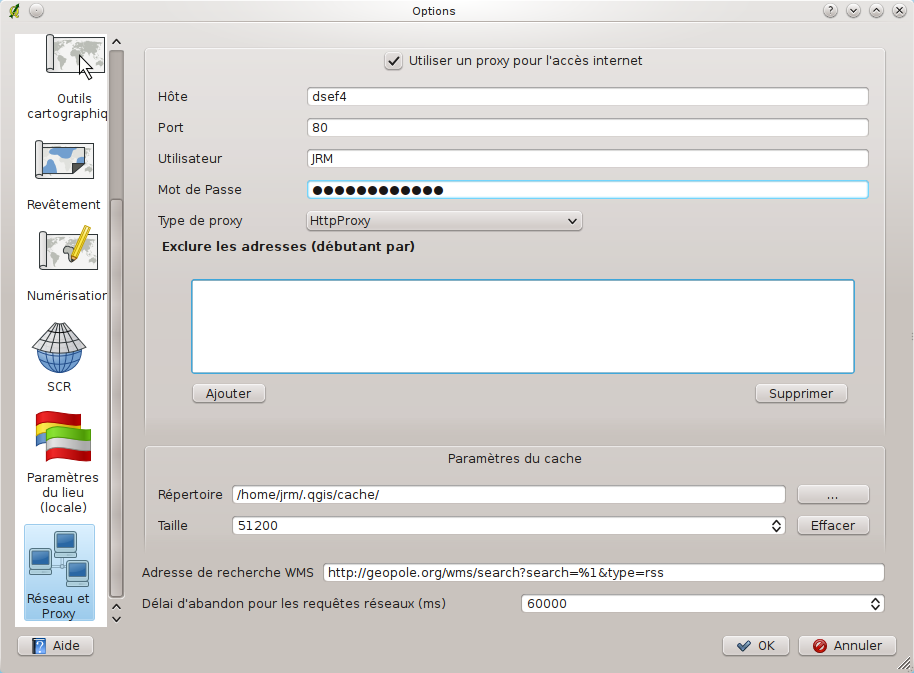
\includegraphics[clip=true, width=14cm]{proxy-settings}
   \caption{Настройка прокси в \qg \nixcaption}
   \label{fig:proxy-settings}
\end{figure}

\begin{Tip} \caption{\textsc{Использование прокси-серверов}}
Использование прокси-серверов иногда может быть довольно сложным. Для проверки вышеописанных типов прокси, действуйте методом <<проб и ошибок>>, проверяя в каждом случае успешность соединений.
\end{Tip}

Можно настроить параметры в соответствии с вашими потребностями. Внесение некоторых изменений, может потребовать перезапуска QGIS, для вступления изменений в силу.

\begin{itemize}
\item \nix{параметры сохраняются в текстовом файле: \$HOME/.config/QuantumGIS/qgis.conf}
\item \osx{ваши настройки можно найти в файле: \$HOME/Library/Preferences/org.qgis.qgis.plist}
\item \win{параметры хранятся в ветке системного реестра:}
\begin{verbatim}
\\HKEY\CURRENT\USER\Software\QuantumGIS\qgis
\end{verbatim}
\end{itemize}

\section{Инструменты аннотации}\label{sec:annotations}
\index{annotations}
\index{text annotation|\see{annotations}}

Инструмент 
\includegraphics[width=0.7cm,clip=true]{mActionTextAnnotation} Текстовая аннотация на панели атрибутов, предоставляет возможность размещения форматированного текста в выноске на карте QGIS. Выберите инструмент аннотаций и нажмите внутри окна карты.

\begin{figure}[ht]
   \centering
   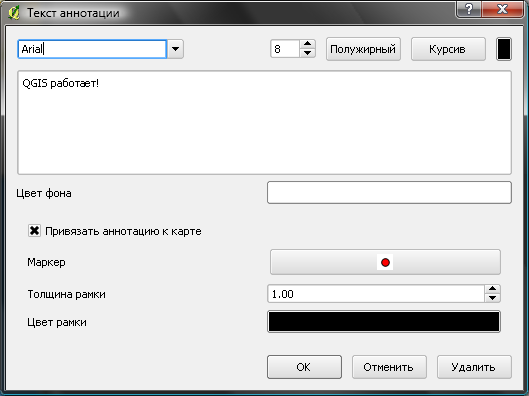
\includegraphics[clip=true, width=12cm]{annotation}
   \caption{Диалоговое окно текста аннотации \nixcaption}
   \label{fig:annotation}
\end{figure}

Двойное нажатие на сноске открывает диалоговое окно с различными параметрами. Здесь находится текстовый редактор для ввода форматированного текста и прочие настраиваемые параметры. Например, можно привязать аннотацию к карте (обозначив маркером) или располагать ее свободно относительно карты. Аннотацию можно перемещать относительно карты (перетаскиванием маркера) или перемещать саму сноску.

Инструмент Переместить аннотацию 
\includegraphics[width=0.7cm,clip=true]{mActionAnnotation} позволяет перемещать аннотацию в окне карты.

\minisec{Диалоговая аннотация}\index{annotations}
\index{form annotation|\see{annotations}}

Дополнительно, вы можете создавать свои собственные диалоговые аннотации. Инструмент Диалоговая аннотация

\includegraphics[width=0.7cm,clip=true]{mActionFormAnnotation} полезен для отображения атрибутов векторного слоя в виде индивидуальной формы, настроенной в qt designer (см. Рисунок \ref{fig:custom-annotations}). Это похоже на конструктор форм для инструмента Определить объекты, но отображается в виде аннотации.
Для получения дополнительной информации, посетите блог QGIS \url{http://blog.qgis.org/node/143}.

\begin{figure}[ht]
   \centering
   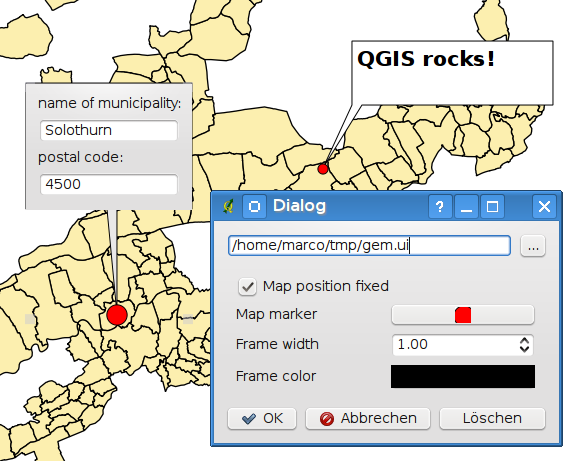
\includegraphics[clip=true, width=10cm]{custom_annotation}
   \caption{Настраиваемая диалоговая аннотация \nixcaption}
   \label{fig:custom-annotations}
\end{figure}

\newpage

\section{Пространственные закладки}\label{sec:bookmarks}
\index{bookmarks}
\index{spatial bookmarks|\see{bookmarks}}

Пространственные закладки позволяют создавать своеобразные <<закладки>> географического положения и возвращаться к ним позднее.

\subsection{Создание закладки}
Для создания закладки:
\begin{enumerate}
\item Масштабируйте или панорамируйте карту до интересующей вас территории.
\item Выберите пункт меню \mainmenuopt{Вид} > \dropmenuopt{Новая закладка} или нажмите \keystroke{Ctrl-B}.
\item Введите описательное имя для закладки (до 255 символов).
\item Нажмите \button{OK}, чтобы добавить закладку, или \button{Отменить} для выхода без добавления закладки.
\end{enumerate}

Помните, что можно иметь множество закладок с одинаковыми названиями.

\subsection{Работа с закладками}
Для использования или управления закладками, выберите пункт меню \mainmenuopt{Вид} > \dropmenuopt{Показать закладки}. Диалоговое окно \\
\dialog{Пространственные закладки} позволяет просматривать или удалять закладки. Но, нельзя редактировать название закладки или координаты.

\subsection{Просмотр закладки}
В диалоговом окне \dialog{Пространственные закладки}, выберите необходимую закладку нажав на ней, затем нажмите кнопку \button{Увеличить до}. Также можно просмотреть закладку дважды нажав на ней.

\subsection{Удаление закладки}
Для удаления закладки из диалогового окна \dialog{Пространственные закладки}, выберите ее и нажмите кнопку \button{Удалить}. Подтвердите ваш выбор нажатием на кнопке \button{ОК} или отмените удаление нажатием кнопки \button{Отменить}.

\section{GPS-слежение}\label{sec:gpstracking}

Для включения GPS-слежения в QGIS необходимо выбрать \mainmenuopt{Вид} > \dropmenuopt{GPS-слежение}. Появится новое пристыкованное окно с левой стороны рабочей области.

Существует 4 варианта экранов этого окна GPS-слежения (см. Рисунок \ref{fig:gpstrack_live}).

\begin{description}
 \item[(a)] 
\includegraphics[width=0.5cm,clip=true]{mActionToggleEditing}
Координаты текущего местоположения и кнопки добавления вершин и объектов
 \item[(b)] 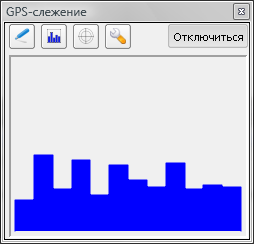
\includegraphics[width=0.5cm,clip=true]{gpstrack_barchart}
Мощность сигнала присоединенных спутников GPS
 \item[(c)] 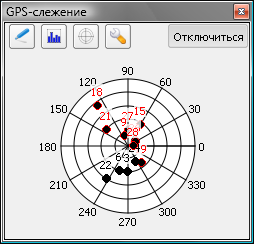
\includegraphics[width=0.5cm,clip=true]{gpstrack_polarchart}
Экран положения спутников GPS, отображающий количество и расположение спутников
 \item[(d)] 
\includegraphics[width=0.5cm,clip=true]{mActionOptions}
Экран параметров GPS (см. Рисунок \ref{fig:gpstrack_options}).
\end{description}

С подключенным GPS-приемником (должен поддерживаться вашей операционной системой), простое нажатие на кнопке \button{Подключиться} подключает GPS к QGIS. Второе нажатие на кнопке (теперь уже \button{Отключиться}) отключает GPS-приемник от компьютера.

[ ВАЖНО ]: Если вы хотите записать текущее местоположение или путь, необходимо сначала создать новый векторный слой и переключиться в режим редактирования.

\begin{figure}[ht]
\centering
   \subfloat[Координаты текущего местоположения] {\label{subfig:gpstrack_main}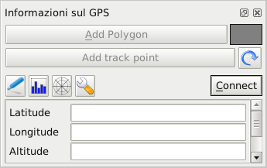
\includegraphics[clip=true, width=0.3\textwidth]{gpstrack_main}}
     \hspace{0.33cm}
   \subfloat[Мощность сигнала GPS]{\label{subfig:gpstrack_stren}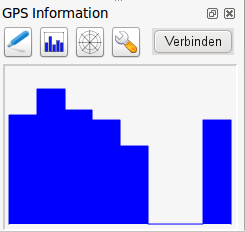
\includegraphics[clip=true, width=0.3\textwidth]{gpstrack_stren}}
     \hspace{0.33cm}
   \subfloat[Положение спутников GPS]{\label{subfig:gpstrack_polar}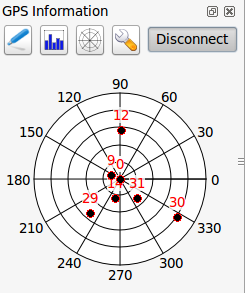
\includegraphics[clip=true, width=0.3\textwidth]{gpstrack_polar}} \\
\end{figure}

\subsection{Координаты текущего местоположения}

\includegraphics[width=0.5cm,clip=true]{mActionToggleEditing} Если GPS-приемник получает сигнал со спутников, вы увидите ваше текущее положение в формате широты и долготы, а также высоту над уровнем моря, как показано на Рисунке \ref{subfig:gpstrack_main}

\subsection{Мощность сигнала GPS}
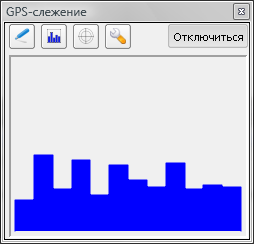
\includegraphics[width=0.5cm,clip=true]{gpstrack_barchart} Здесь можно видеть мощность сигнала спутников, с которых вы получаете сигнал (Рисунок \ref{subfig:gpstrack_stren}).

\subsection{Положение спутников GPS}
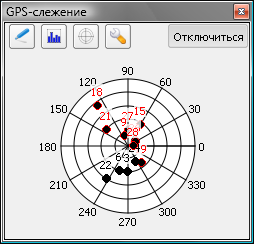
\includegraphics[width=0.5cm,clip=true]{gpstrack_polarchart} Если вы хотите знать, где на небесной сфере располагаются все присоединенные спутники, переключитесь на окно Положение спутников (Рисунок \ref{subfig:gpstrack_polar}). Также здесь можно увидеть идентификационные номера (ID) спутников, с которых вы получаете сигнал.

\subsection{Параметры GPS}

\includegraphics[width=0.5cm,clip=true]{mActionOptions} В случае возникновения проблем с соединением, можно переключиться с \radiobuttonon{{}Автоопределение} на \radiobuttonon{{}Использовать указанный путь}, и выбрать путь (и порт) присоединенного GPS-приемника. Нажатие кнопки \button{Подключиться} снова инициирует соединение с GPS-приемником.

Ползунком \slider{Размер курсора} можно уменьшать и увеличивать курсор текущего местоположения в окне карты. Включение параметра \radiobuttonon{{}Автоматически создавать вершины} в Оцифровке, будет автоматически записывать трек в активный векторный слой (разумеется, слой должен быть в режиме редактирования).

Установка параметра центрирования карты позволяет контролировать, в каких случаях будет обновляться окно карты: в случае, если записываемые координаты выходят за текущий охват карты, либо всегда (или же никогда).

Параметр Цвет трека задает цвет и толщину отрисовываемого трека.

Если вы хотите добавлять объекты вручную, вернитесь обратно к окну 
\includegraphics[width=0.5cm,clip=true]{mActionToggleEditing} <<Координаты текущего местоположения>> и нажмите
\button{Добавить объект}. Также, если не активна функция <<Автоматически создавать вершины>> и вы хотите создавать вершины вручную, нажмите \button{Добавить вершину}

\begin{figure}[ht]
   \centering
   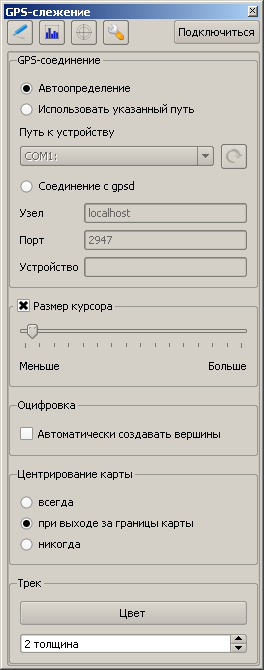
\includegraphics[clip=true, width=5cm]{gpstrack_options}
   \caption{Окно параметров GPS-слежения \nixcaption}
   \label{fig:gpstrack_options}
\end{figure}

\FloatBarrier
